\documentclass{bmstu}

\bibliography{biblio}

\renewcommand\labelitemi{---}
\renewcommand\labelitemii{---}

\usepackage{listingsutf8}
\lstset{columns=fixed,basicstyle=\small,breaklines=true,inputencoding=utf8,keywordstyle=\bfseries\underbar,frame=single,tabsize=2,xleftmargin=20pt,xrightmargin=5pt}
\lstset{language=sql}
\lstset{numbers=left,numberstyle=\small}

\lstset{extendedchars=\true}

\usepackage{pdfpages}

\geometry{a4paper,left=3.1cm,right=1.1cm,top=2cm,bottom=2cm,bindingoffset=0cm}

\begin{document}

\makeresearchtitle{Информатика и системы управления}{Программное обеспечение ЭВМ и информационные технологии}{Классификация запросов в предметной области на примере анализа запросов к базам данных}{А.~В.~Княжев/ИУ7-72Б}{Ю.~В.~Строганов}{}{}

%\includepdf{assets/task.pdf}
\setcounter{page}{3}

\begin{essay}{}

\textbf{Ключевые слова:} базы данных, языки запросов, Prolog, SQL, ORM.

В данной работе проведен обзор существующих видов запросов в произвольной предметной области, обзор систем управления базами данных PostgreSQL и Greenplum. Кроме того, проведен опрос, позволяющий определить среднее время ответа респондентов и процент ошибок в вопросах, связанных с запросами к базе данных на SQL, Prolog/Datalog и ORM. По результатам опроса выявлено, что вопросы с Prolog/Datalog занимают в среднем меньшее время на заданной выборке респондентов.

\end{essay}
\maketableofcontents
\begin{definitions}
	\definition{Система управления базами данных}{это набор программ, которые управляют структурой БД и контролируют доступ к данным, хранящимся в БД~\cite{швецов2009базы}.}
	\definition{Сериализация}{процесс перевода структуры в текстовый формат, предназначенный для обмена информацией между существенно отличающимися друг от друга программными системами.~\cite{погодин2018сериализация}}
\end{definitions}
\begin{abbreviations}
	\definition{FD}{File Descriptor~\cite{dumitran2007fixing}.}
	\definition{HTTP}{HyperText Transfer Protocol~\cite{fielding2022rfc}.}
	\definition{TCP}{Transmission Control Protocol~\cite{eddy2022rfc}.}
\end{abbreviations}

\chapter*{ВВЕДЕНИЕ}
\addcontentsline{toc}{chapter}{ВВЕДЕНИЕ}

Ежегодно кафедра ИУ7 проводит конкурс «Шаг в будущее» для абитуриентов в соотвествии с положением и регламентом проведения данного конкурса \cite{bib1, bib2}. Конкурс в 2023 году был проведен 24 марта. Организаторы конкурса согласованы в документе состава оргкомитета \cite{bib3}, а также все организационные материалы и члены жюри олимпиады «Шаг в будущее» утверждены в соответствующих документах \cite{bib4, bib5}.

\textbf{Цель практики}~---~организация проектного этапа олимпиады <<Шаг в будущее~---~2023>> МГТУ им. Н.Э. Баумана, секции кафедры ИУ-7 в форме программного салона.

Для достижения поставленной цели необходимо решить следующие задачи.

\begin{enumerate}
	\item Установить ПО, необходимое для демонстрации работы проектов участников.
	\item Изучить работу участников.
	\item Составить студенческие рецензии.
	\item Произвести обзвон участников.
	\item Поучаствовать в очной оценке работ.
\end{enumerate}

\chapter{Аналитический раздел}

\section{Анализ предметной области}
С увеличением числа сотрудников компании часто возникают проблемы внутренней коммуникации сотрудников, получения информации о коллегах и автоматизации процессов рекрутмента~\cite{intranet_avito}. Для решения этих задач существуют внутренние порталы для сотрудников. Обычно они представляют функционал, схожий с соцсетями: отображение профилей пользователей, и др. 

В основном, внутренние порталы для сотрудников представляют собой закрытые решения~\cite{глухих2005глухих}, которые разрабатываются в рамках одной компании~\cite{rivelty}, и не распространяются во внешний мир вследствии политики конфиденциальности~\cite{klee2000importance}. 



\section{Сравнение с аналогичными решениями}
В данной части проводится сравнение предлагаемого решения с аналогами~---~наиболее активно используемыми и разрабатываемыми известными внутренними порталами для сотрудников~\cite{rivelty}.

\paragraph{Критерии сравнения} \mbox{}

В качестве критериев сравнения решений были выбраны основные элементы функционала:

\begin{enumerate}
	\item возможность просматривать профили пользователей;
	\item хранение информации об иерархии сотрудников;
	\item возможность хранить информацию о команде сотрудника;
	\item отсутствие платы за использование;
	\item открытость решения для использования.
\end{enumerate}


\paragraph{Сравнение} \mbox{}

В таблице \ref{table:anal_compare} приведено сравнение решений для внутреннего портала для сотрудников организации.

\begin{table}[h]
  \caption{\label{table:anal_compare} Сравнение существующих решений с предложенным}
  \begin{center}
    \begin{tabular}{|l|l|l|l|l|l|}
      \hline
      Решение              & 1 & 2 & 3 & 4 & 5 \\ \hline
      Интранет VK~\cite{intranet_vk}          & $+$ & $+$ & $-$ & $+$ & $-$ \\ \hline
      Avito People~\cite{intranet_avito}         & $+$ & $+$ & $+$ & $+$ & $-$ \\ \hline
      Битрикс24~\cite{bitrix24}           & $+$ & $+$ & $-$ & $-$ & $+$ \\ \hline
      Предлагаемое решение & $+$ & $+$ & $+$ & $+$ & $+$ \\ \hline
    \end{tabular}
  \end{center}
\end{table}

\section{Формализация задачи}
Решение должно представлять собой портал, в котором будет производиться регистрация сотрудника менеджером по персоналу. Сотрудник сможет просматривать профили других сотрудников, производить поиск по организации.

Каждый сотрудник состоит в некоторой иерархии: у него есть руководитель и подразделение, в котором он находится. Кроме того, роль сотрудника может не совпадать с его положением в этой иерархии~\cite{intranet_avito}. Например, по документам он может находиться в департаменте разработки, а фактически находиться в команде какого-либо проекта. Решение должно учитывать эту особенность.

Сотрудник может редактировать основные данные профиля: фотографию, описание профиля, информацию об отпуске, при этом такую информацию, как имя, должность и положение в иерархии компании может изменять только рекрутер.


\paragraph{Формализация сценариев использования} \mbox{}

В рамках решения должно существовать три вида пользователей:

\begin{enumerate}
	\item Сотрудник~---~сотрудник предприятия. Имеет базовые возможности по изменению части информации профиля, поиску среди пользователей системы.
	\item Рекрутер~---~менеджер по персоналу. Может создавать профили сотрудников, удалять их, изменять базовую информацию, такую как имя, должность.
	\item Администратор~---~главная роль в системе. Может делать то же, что может рекрутер. Кроме того, может редактировать базовую структуру организации, и управлять другими администраторами.
\end{enumerate}

На рис.~\ref{img:use-case} изображена диаграмма сценариев использования предлагаемого решения.

\begin{figure}[h!]
\centering
    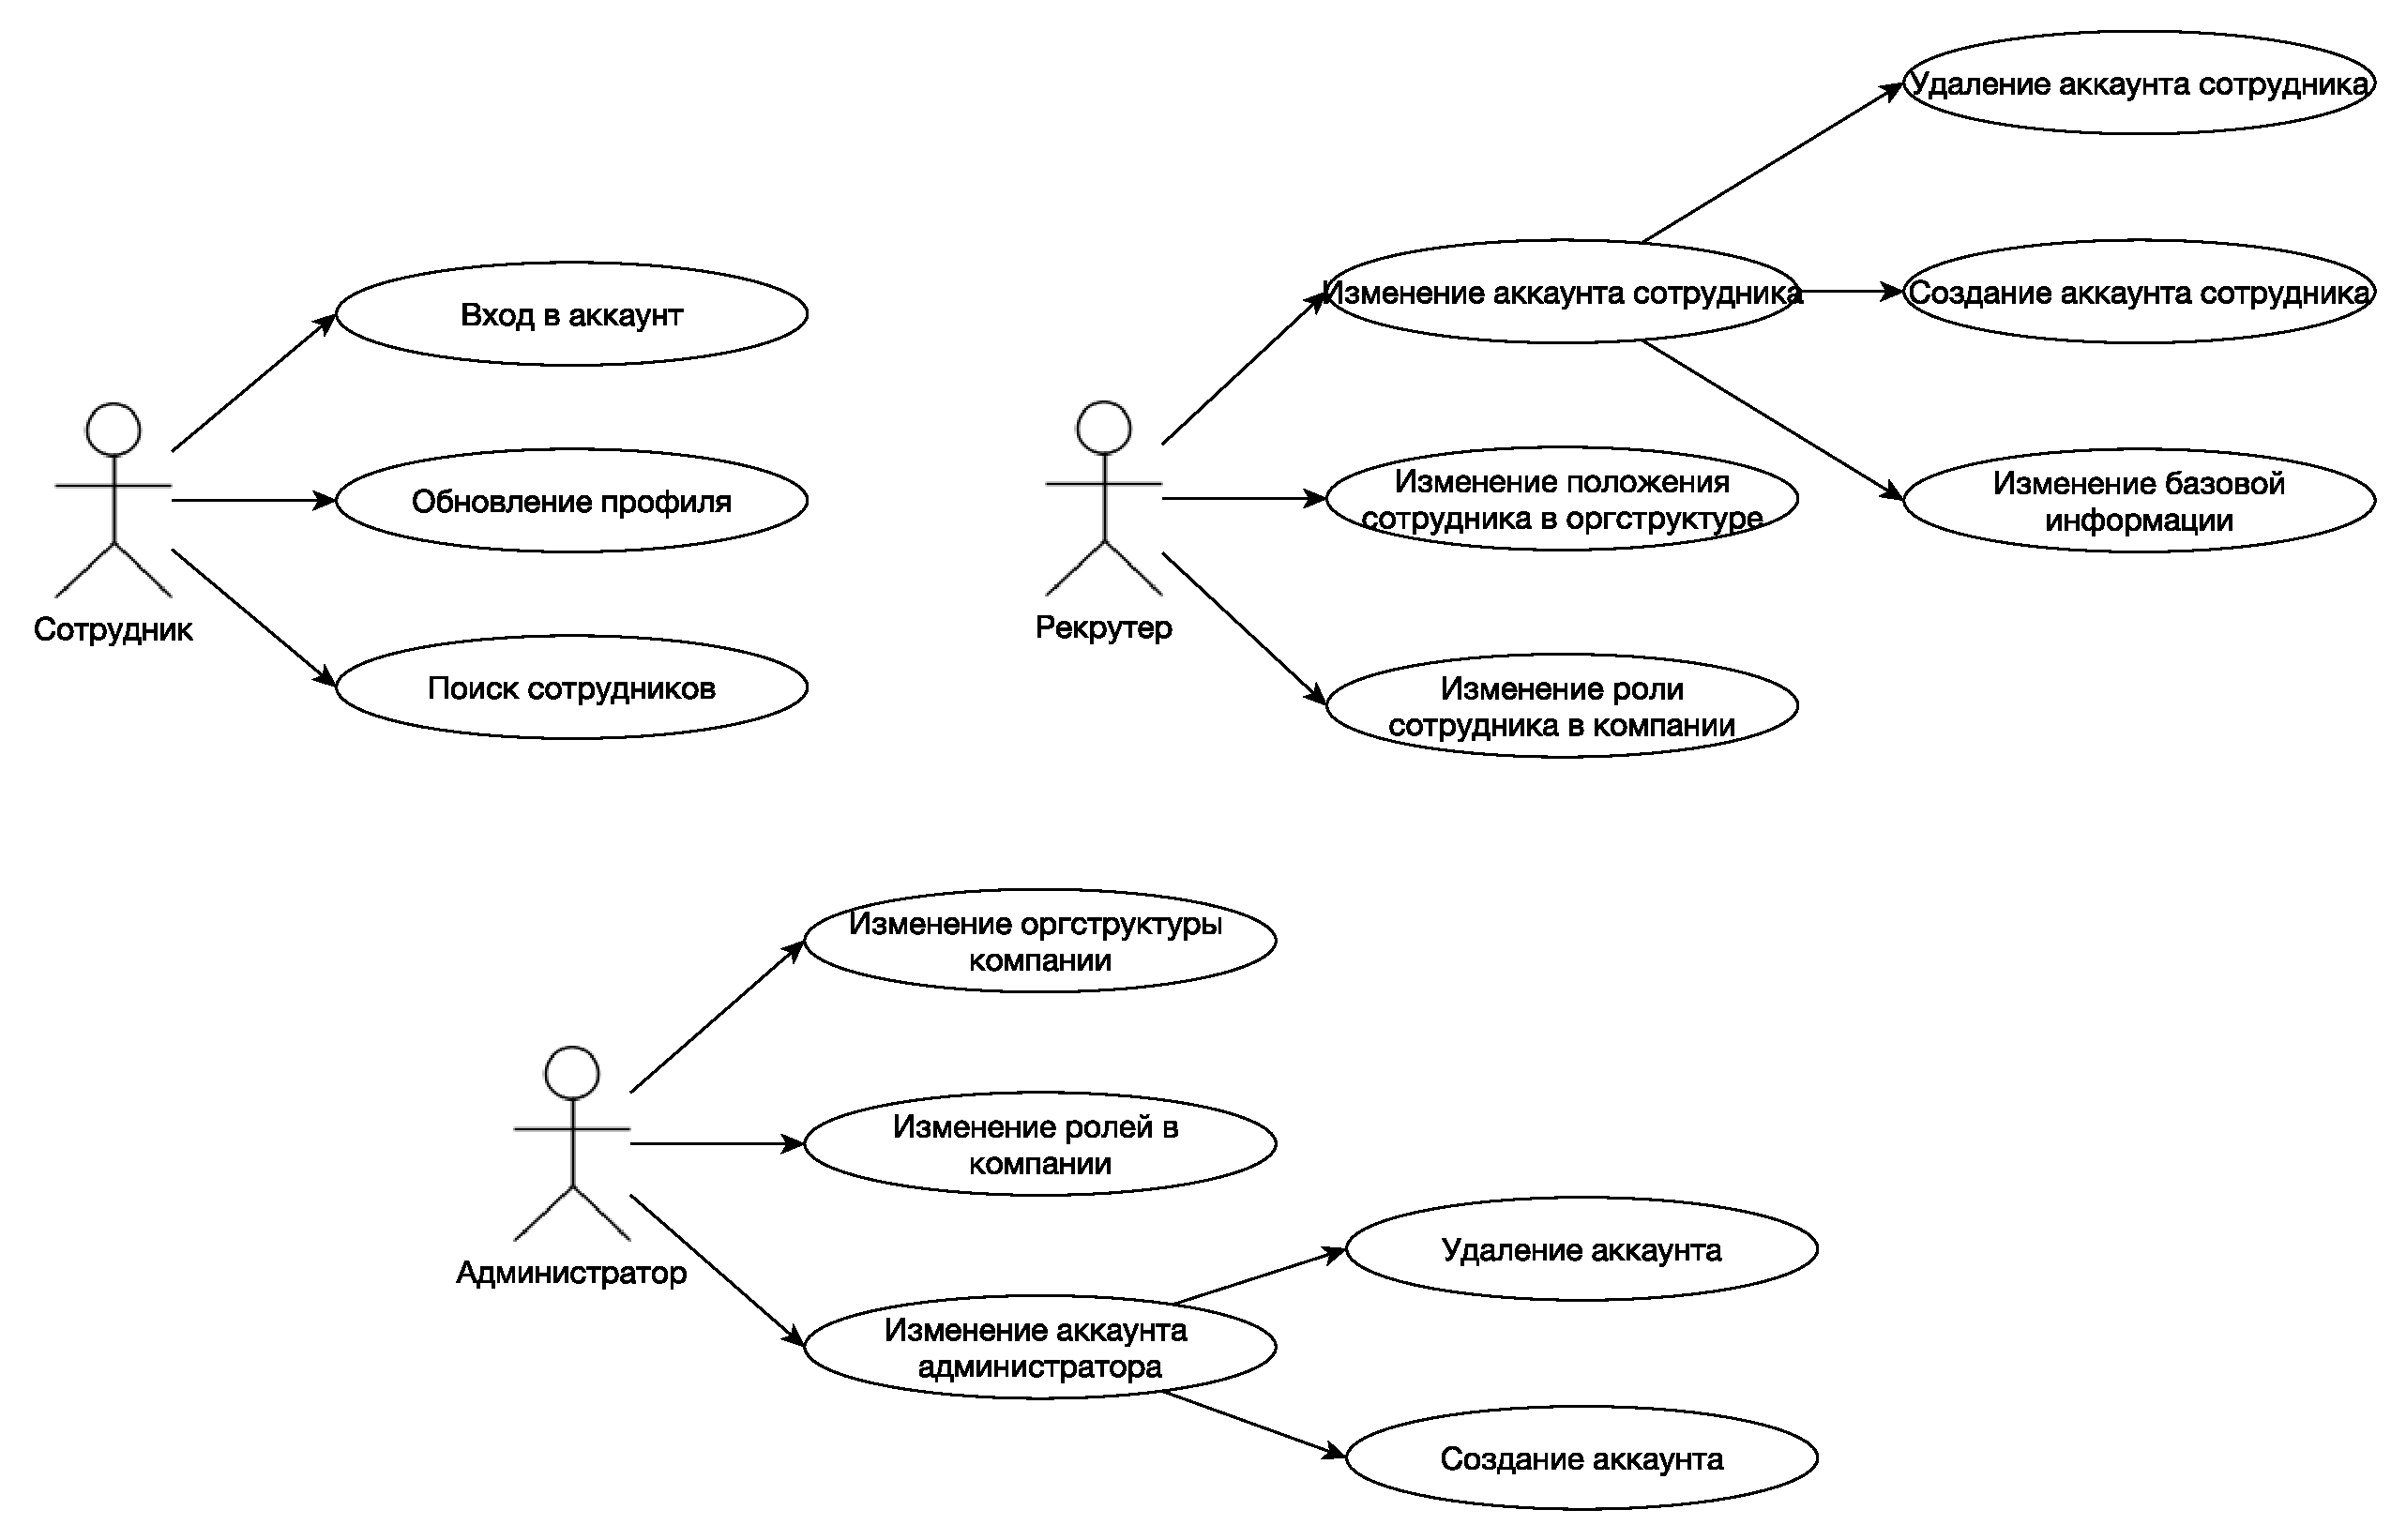
\includegraphics[width=0.9\linewidth]{assets/use-case.pdf}
    \caption{Диаграмма сценариев использования (начало)}
    \label{img:use-case}	
\end{figure}

%\begin{figure}[h!]
%\centering
%    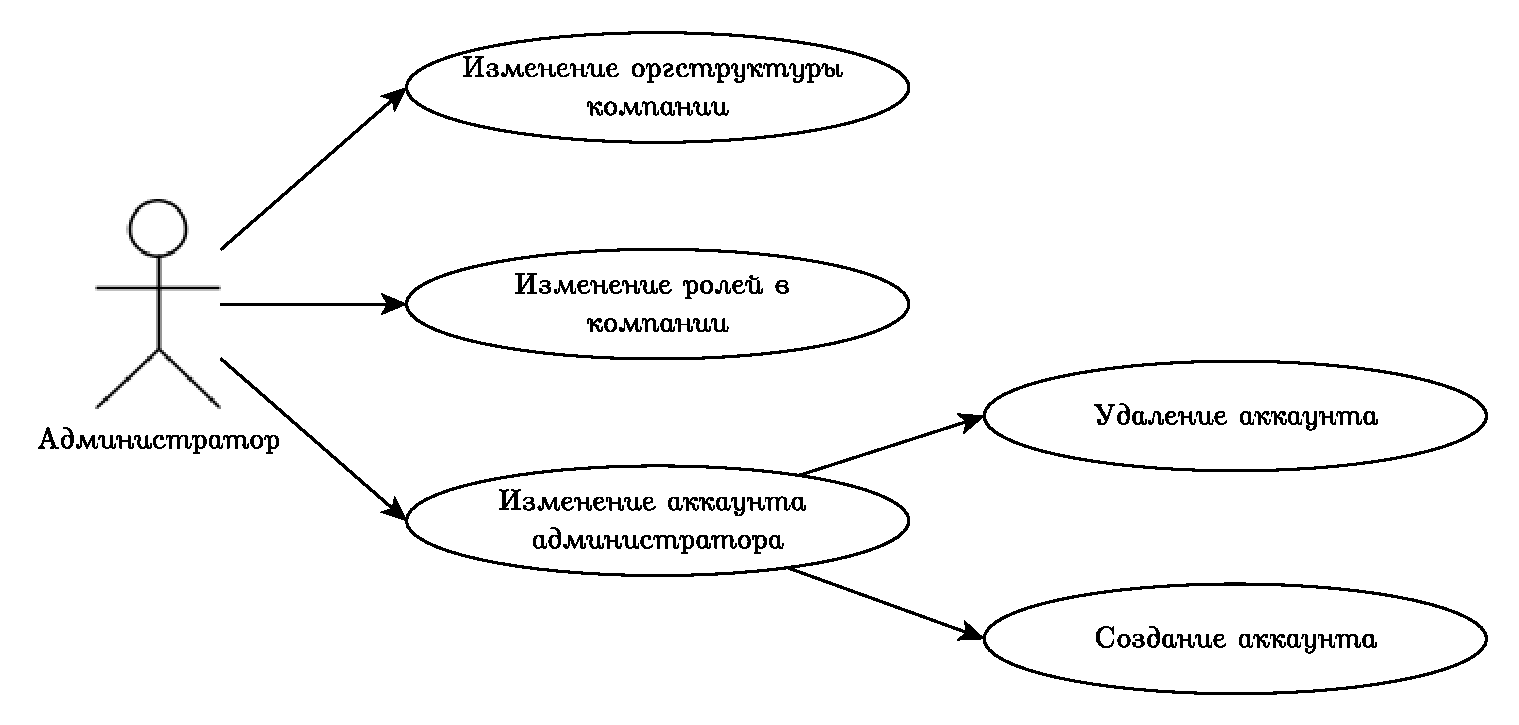
\includegraphics[width=0.8\linewidth]{assets/use-case1.pdf}
%    \caption{Диаграмма сценариев использования (конец)}
%    \label{img:use-case1}	
%\end{figure}


\paragraph{Формализация данных} \mbox{}

Основные сущности, которые должны содержаться в проектируемой базе данных:

\begin{itemize}
	\item сотрудник;
	\item команда~---~фактическая команда, в которой работает сотрудник;
	\item подписка;
	\item отпуск;
	\item отдел~---~официальный департамент, в который трудоустроен сотрудник.
\end{itemize}

На рис.~\ref{img:chen} изображена ER-диаграмма сущностей проектируемой базы данных в нотации Чена.

\newpage

\begin{figure}[h!]
\centering
    \includegraphics[width=0.9\linewidth]{assets/chen.pdf}
    \caption{ER-диаграмма сущностей в нотации Чена}
    \label{img:chen}	
\end{figure}


\section{Виды СУБД по модели данных}

База данных представляет собой набор связанных данных некоторой предметной области, поэтому для ее организации важно определиться с моделью данных. Модель данных представляет собой логическую структуру данных, хранящихся в базе данных~\cite{хомоненко2000базы}. На данный момент, в качестве основных моделей данных выделяют дореляционные, реляционные и нереляционные.

\paragraph{Дореляционные} \mbox{}

Дореляционные базы данных не основываются на абстрактных моделях, доступ осуществляется на уровне записей~\cite{бородин2016задаче}. 

Среди дореляционных моделей можно выделить~\cite{дадян2016методы}:
\begin{itemize}
	\item Иерархическая~---~представлена в базе данных в виде дерева~\cite{корягин2020модели}.
	\item Сетевая~---~является расширением иерархической БД. У потомка может быть больше одного родителя. Такая модель поддерживает отношение «многие-ко-многим»~\cite{корягин2020модели}. 
\end{itemize}

Среди особенностей дореляционных моделей можно отметить сложность использование и зависимость прикладных программ от физической реализации СУБД~\cite{бородин2016задаче}. 

\paragraph{Реляционные} \mbox{}

Реляционная база данных~---~совокупность отношений, содержащих всю информацию, которая должна храниться в базе данных~\cite{кириллов2012введение}. В основном воспринимаются как базы, в которых данные хранятся в двумерных таблицах, а установленная между ними связь позволяет избегать повторения данных~\cite{жалолов2020понятие}.


Таблица реляционной базы данных устроена следующим образом. Столбец таблицы представляет собой поле~---~значение атрибута отношения. Строка представляет собой конкретную запись, кортеж этого отношения. Такая структура позволяет создать наиболее простое и понятное пользователю представление базы данных, при такой организации данные хорошо структурированы~\cite{бородин2016задаче}. 


\paragraph{Нереляционные} \mbox{}

Нереляционные модели убирают строгие связи между данными в системе. Нереляционные базы данных бывают~\cite{бородин2016задаче}:

\begin{itemize}
	\item колоночные;
	\item документоориентированные;
	\item вида ключ-значение;
	\item графовые;
	\item с другие.
\end{itemize}

Основными отличиями от реляционной модели являются меньшая структуризация, отсутствие стандартизации~\cite{корягин2020модели}.

В данном разделе была проведена формализация задачи: рассмотрена предметная область, формализованы данные и сценарии использования. Проведено сравнение с конкурентами по основным критериям.

Кроме того, рассмотрены виды СУБД по модели данных. В связи с отсутствием необходимости специфичной обработки данных и необходимостью структурировать данные, была выбрана реляционная модель.

 
\chapter{Обзор СУБД PostgreSQL и Greenplum}

В данной части рассматриваются системы управления базами данных PostgreSQL и Greenplum. PostgreSQL на текущий момент является одной из самых популярных СУБД в мире, и в России в частности~\cite{штомпель2019вакансия}. При этом, данная СУБД не обладает такими функциями, как автоматическое восстановление кластера после сбоев, для чего существуют такие внешние инструменты, как Patroni~\cite{kumar2021postgresql}. Greenplum использует в качестве своих рабочих узлов СУБД PostgreSQL, при этом реализует недостающий в PostgreSQL функционал по работе в кластерном режиме, например, автоматическое восстановление и распределенные транзакции~\cite{lyu2021greenplum}.

\section{PostgreSQL}

PostgreSQL~---~объектно-реляционная система управлениями базами данных с открытым исходным кодом~\cite{makris2021mongodb}. Обладает следующими возможностями~\cite{drake2002practical}.

\begin{itemize}
	\item \textbf{Пользовательские операции и функции.} В БД поддерживается объявление пользовательских операций, функций, процедур и типов данных.
	\item \textbf{Поддержка языка SQL.} Поддерживается весь стандартный синтаксис языка SQL. Кроме того, имеются специфичные для PostgreSQL расширения языка.
	\item \textbf{Принципы ACID.} PostgreSQL является транзакционной базой данных~---~OLTP, соответственно, поддерживает принципы атомарности, целостности, изолированности и надежности.
	\item \textbf{Расширяемый API.} Для PostgreSQL можно создавать дополнения на разных языках программирования. Эти дополнения позволяют расширять стандартный функционал базы данных. Например, расширение PostGIS добавляет поддержку работы с геоданными~\cite{obe2021postgis}.
	\item \textbf{Интеграция процедурных языков программирования.} Кроме языка SQL, для работы с данными в базе данных могут быть использованы некоторые процедурные языки программирования, например, Python, Perl и другие.
	\item \textbf{Клиент-серверная архитектура.} PostgreSQL использует клиент-серверную архитектуру. Основной процесс создает дочерний процесс для обработки клиентского соединения.
	\item \textbf{WAL.} После каждой операции с базой данных, еще до изменения данных на диске, происходит запись в лог. Этот лог используется для повышения отказоустойчивости базы данных, так как он может послужить опорной точкой для восстановления данных в случае аварийного завершения работы СУБД. Кроме того, лог используется для репликации базы данных.
	\item \textbf{Репликация.} В PostgreSQL реализованы две стратегии репликации: синхронная и асинхронная. В случае синхронной репликации, изменения данных с основной реплики копируются на реплики-копии сразу после изменения данных. В случае асинхронной репликации, изменения будут скопированы только после применения всей транзакции на основной реплике~\cite{boszormenyi2013postgresql}.
\end{itemize}



\section{Greenplum}


Greenplum~---~масштабируемая система для организации хранилища данных.  Обладает следующими возможностями~\cite{lyu2021greenplum}.

\begin{itemize}
	\item \textbf{Массивно-параллельная архитектура.} Greenplum разделяет данные на фрагменты, которые хранит на рабочих узлах. Запрос к данным выполняется сначала на сегментах, затем результат от сегментов агрегируется на основном узле.
	\item \textbf{Разделение сегментов.} Узлы кластера Greenplum не разделяют память и другие ресурсы. Обмен данными между ними происходит только по сети.
	\item \textbf{Репликация.} У узлов кластера могут быть так называемые «узлы-зеркала»~---~узлы, не участвующие в выполнении запросов, но получающие обновления WAL с основных узлов.
	\item \textbf{Распределенные транзакции.} Для выполнения принципов ACID в рамках распределенной системы, в Greenplum реализован двухфазный протокол применения транзакции.
\end{itemize}



\chapter{Сравнение способов составления запросов к базам данных}

В данной части производится сравнение способов составления запросов к базам данных.

\begin{enumerate}
	\item SQL.
	\item Prolog/Datalog.
	\item ORM.
\end{enumerate}

Для способов составления запросов может быть выявлен критерий «понятности». В данном случае, в качестве критерия «понятности» можно использовать процент ошибок, совершенный человеком при распознавании запроса и время, затраченное на распознавание. Чем процент ошибок и время меньше~---~тем более «понятным» можно считать способ.

Для получения значения количества ошибок и времени ответа проведен опрос, в котором участники могут выбрать вариант ответа базы данных на указанный запрос. В качестве базы данных для опроса используется тестовая база данных Northwind~\cite{dyer2015adapting}.

\section{Проведение опроса}

Для оценки количества ошибок составляется тест, состоящий из 21 вопросов, по 7 вопросов на каждый из способов. Вопрос представляет собой запрос с использованием одного из способов к базе данных и 8 вариантов ответа. Вопросы и варианты ответа на них приведены в Приложении~А.

Для оценки времени ответа на вопрос, используется среднее значение 75-ых перцентилей времени ответа на каждый запрос, заданный с помощью одного из способов составления запроса. Результаты опроса сгруппированы по связи респондентов со сферой информационных технологий и по виду использования связей: запросы одной или нескольких сущностей.

Результаты времени ответа на запросы одной сущности респондентов, работа или учеба которых связана с информационными технологиями, следующие:

\begin{itemize}
	\item \textbf{SQL}~---~63 секунды;
	\item \textbf{Prolog/Datalog}~---~46 секунд;
	\item \textbf{ORM}~---~63 секунды.
\end{itemize}

Результаты времени ответа на запросы нескольких сущностей респондентов, работа или учеба которых связана с информационными технологиями, следующие:

\begin{itemize}
	\item \textbf{SQL}~---~141 секунда;
	\item \textbf{Prolog/Datalog}~---~134 секунды;
	\item \textbf{ORM}~---~158 секунд.
\end{itemize}

Результаты времени ответа на запросы одной сущности респондентов, работа или учеба которых не связана с информационными технологиями, следующие:

\begin{itemize}
	\item \textbf{SQL}~---~73 секунды;
	\item \textbf{Prolog/Datalog}~---~38 секунд;
	\item \textbf{ORM}~---~76 секунд.
\end{itemize}

Результаты времени ответа на запросы нескольких сущностей респондентов, работа или учеба которых не связана с информационными технологиями, следующие:

\begin{itemize}
	\item \textbf{SQL}~---~154 секунды;
	\item \textbf{Prolog/Datalog}~---~126 секунд;
	\item \textbf{ORM}~---~191 секунд.
\end{itemize}

Для оценки правильности ответа используется процент ошибок на вопросы, составленные с помощью одного из способа составления запроса. 

Результаты процента ошибок на запросы одной сущности респондентов, работа или учеба которых связана с информационными технологиями, следующие:

\begin{itemize}
	\item \textbf{SQL}~---~22\%;
	\item \textbf{Prolog/Datalog}~---~25\%;
	\item \textbf{ORM}~---~23\%.
\end{itemize}

Результаты процента ошибок на запросы нескольких сущностей респондентов, работа или учеба которых связана с информационными технологиями, следующие:

\begin{itemize}
	\item \textbf{SQL}~---~52\%;
	\item \textbf{Prolog/Datalog}~---~46\%;
	\item \textbf{ORM}~---~45\%.
\end{itemize}

Результаты процента ошибок на запросы одной сущности респондентов, работа или учеба которых не связана с информационными технологиями, следующие:

\begin{itemize}
	\item \textbf{SQL}~---~64\%;
	\item \textbf{Prolog/Datalog}~---~60\%;
	\item \textbf{ORM}~---~60\%.
\end{itemize}

Результаты процента ошибок на запросы нескольких сущностей респондентов, работа или учеба которых не связана с информационными технологиями, следующие:

\begin{itemize}
	\item \textbf{SQL}~---~59\%;
	\item \textbf{Prolog/Datalog}~---~67\%;
	\item \textbf{ORM}~---~75\%.
\end{itemize}

%\section{Определение предметной области}
%
%В качестве примера будет использоваться предметная область исследования времяпрепровождения клиентов некоторого концерна по производству пива и закусок к нему.
%
%Составленная база данных будет использована для хранения ответов аудитории на социальный опрос, целью которого будет выяснить, какое сочетания пива, закуски и фильма клиент считает наилучшим времяпрепровождением для себя.
%
%Рассматриваемая база данных состоит из следующих сущностей.
%
%\begin{itemize}
%	\item \textbf{Пиво}~---~конкретная серия пива некоторого производителя.
%	\item \textbf{Производитель пива}~---~пивоваренная компания.
%	\item \textbf{Описание пива}~---~описание основных характеристик пива. Включает в себя описание, состав и крепость в процентах.
%	\item \textbf{Фильм}~---~конкретный фильм, который предпочитает смотреть аудитория.
%	\item \textbf{Модель чипсов}~---~серия чипсов без привязки ко вкусу.
%	\item \textbf{Вкус чипсов}~---~вкус чипсов без привязки к серии.
%\end{itemize}
%
%База данных составлена таким образом, чтобы она содержала все вышеуказанные виды отношений между сущностями.
%
%\begin{enumerate}
%	\item \textbf{Один-к-одному:} связь между пивом и его описанием
%	\item \textbf{Один-ко-многим:} связь между производителем пива и непосредственно пивом.
%	\item \textbf{Многие-ко-многим:} связь между моделью чипсов и вкусом.
%	\item \textbf{n-арная связь:} связь между фильмом, чипсами (включая модель и вкус) и пивом.
%\end{enumerate}
%
%\newpage
%
%На рисунке \ref{img:chen} представлена диаграмма базы данных в нотации Чена.
%
%\begin{figure}[h!]
%\centering
%    \includegraphics[width=1\linewidth]{assets/chen.pdf}
%    \caption{ER-диаграмма сущностей в нотации Чена}
%    \label{img:chen}	
%\end{figure}
%
%\section{Запросы к предметной области}
%
%В данном разделе предложены примеры запросов к предметной области для разных видов отношений и использования связей при работе с БД. Каждый пример в данном случае будет описан на естественном языке, SQL, ORM, Prolog и Datalog. В качестве ORM в данной работе будет рассмотрен GORM.
%
%\subsection{Запрос одной сущности}
%
%Запрос на естественном языке: «Какие фильмы вышли после 2000 года?».
%
%В листинге \ref{lst:1::sql} приведен пример указанного запроса на языке SQL.
%
%\begin{lstlisting}[label=lst:1::sql,caption=Пример листинга на языке SQL]
%select name from film where year > 2000;
%\end{lstlisting}
%
%В листинге \ref{lst:1::orm} приведен пример указанного запроса на ORM.
%
%\begin{lstlisting}[label=lst:1::orm,caption=Пример листинга на ORM]
%db.Table("film").Select("name").Where("year > ?", 2000).Take(&name).Error
%\end{lstlisting}
%
%В листинге \ref{lst:1::prolog} приведен пример указанного запроса на Prolog.
%
%\begin{lstlisting}[label=lst:1::prolog,caption=Пример листинга на языке Prolog]
%film(_,Name,Year), Year > 2000.
%\end{lstlisting}
%
%В листинге \ref{lst:1::datalog} приведен пример указанного запроса на Datalog.
%
%\begin{lstlisting}[label=lst:1::datalog,caption=Пример листинга на языке Datalog]
%TODO!!!
%\end{lstlisting}
%
%\subsection{Запрос нескольких сущностей}
%
%\subsubsection{Отношение один-к-одному}
%
%Запрос на естественном языке: «У какого пива крепость выше 8\%?».
%
%В листинге \ref{lst:some:1-1:sql} приведен пример указанного запроса на языке SQL.
%
%\begin{lstlisting}[label=lst:some:1-1:sql,caption=Пример листинга на языке SQL]
%select name from beer b join beerDescription bd on b.descriptionID = bd.id where bd.alcohol > 8.0;
%\end{lstlisting}
%
%В листинге \ref{lst:some:1-1:orm} приведен пример указанного запроса на ORM.
%
%\begin{lstlisting}[label=lst:some:1-1:orm,caption=Пример листинга на ORM]
%db.Table("beer").Select("beer.name").Join("beerDescription bd on beer.descriptionID = bd.id").Where("bd.alcohol > ?", 8.0).Take(&name).Error
%\end{lstlisting}
%
%В листинге \ref{lst:some:1-1:prolog} приведен пример указанного запроса на Prolog.
%
%\begin{lstlisting}[label=lst:some:1-1:prolog,caption=Пример листинга на языке Prolog]
%beer(_,Name,_,DescriptionID), beerDescription(DescriptionID,_,_,Alcohol), Alcohol > 8.
%\end{lstlisting} 
%
%В листинге \ref{lst:some:1-1:datalog} приведен пример указанного запроса на Datalog.
%
%\begin{lstlisting}[label=lst:some:1-1:datalog,caption=Пример листинга на языке Datalog]
%TODO!!!
%\end{lstlisting}
%
%\subsubsection{Отношение один-ко-многим}
%
%Запрос на естественном языке: «Какие виды пива выпускает компания Балтика?».
%
%В листинге \ref{lst:some:1-n:sql} приведен пример указанного запроса на языке SQL.
%
%\begin{lstlisting}[label=lst:some:1-n:sql,caption=Пример листинга на языке SQL]
%select name from beer b join beerProducer bp on b.producerID = bp.id where bp.name = 'Балтика';
%\end{lstlisting}
%
%В листинге \ref{lst:some:1-n:orm} приведен пример указанного запроса на ORM.
%
%\begin{lstlisting}[label=lst:some:1-n:orm,caption=Пример листинга на ORM]
%db.Table("beer").Select("beer.name").Join("beerProducer bp on beer.producerID = bp.id").Where("bp.name = ?", "Балтика").Take(&name).Error
%\end{lstlisting}
%
%В листинге \ref{lst:some:1-n:prolog} приведен пример указанного запроса на Prolog.
%
%\begin{lstlisting}[label=lst:some:1-n:prolog,caption=Пример листинга на языке Prolog]
%beer(_,Name,ProducerID,_), beerProducer(ProducerID,"Балтика").
%\end{lstlisting} 
%
%В листинге \ref{lst:some:1-n:datalog} приведен пример указанного запроса на Datalog.
%
%\begin{lstlisting}[label=lst:some:1-n:datalog,caption=Пример листинга на языке Datalog]
%TODO!!!
%\end{lstlisting}
%
%\subsubsection{Отношение многие-ко-многим}
%
%Запрос на естественном языке: «Какие есть серии чипсов со вкусом соленых огурцов».
%
%В листинге \ref{lst:some:m-n:sql} приведен пример указанного запроса на языке SQL.
%
%\begin{lstlisting}[label=lst:some:m-n:sql,caption=Пример листинга на языке SQL]
%select c.name from chips c join chipsWithTaste cwt on c.id = cwt.chipsID join chipsTaste on cwt.tasteID = ct.id where ct.name = 'Соленые огурцы';
%\end{lstlisting}
%
%В листинге \ref{lst:some:m-n:orm} приведен пример указанного запроса на ORM.
%
%\begin{lstlisting}[label=lst:some:m-n:orm,caption=Пример листинга на ORM]
%db.Table("chips").Select("chips.name").Join("chipsWithTaste cwt on c.id = cwt.chipsID").Join("chipsTaste on cwt.tasteID = ct.id").Where("ct.name = ?", "Соленые огурцы").Take(&name).Error
%\end{lstlisting}
%
%В листинге \ref{lst:some:m-n:prolog} приведен пример указанного запроса на Prolog.
%
%\begin{lstlisting}[label=lst:some:m-n:prolog,caption=Пример листинга на языке Prolog]
%chips(ChipsID,Name), chipsWithTaste(_,ChipsID,TasteID), chipsTaste(TasteID,"Соленые огурцы").
%\end{lstlisting} 
%
%В листинге \ref{lst:some:m-n:datalog} приведен пример указанного запроса на Datalog.
%
%\begin{lstlisting}[label=lst:some:m-n:datalog,caption=Пример листинга на языке Datalog]
%TODO!!!
%\end{lstlisting}
%
%\subsection{Запрос большого количества сущностей}
%
%\subsubsection{n-арное отношение}
%
%Запрос на естественном языке: «Какие фильмы сочетаются с чипсами Русская картошка со вкусом соленых огурцов и пивом крепостью выше 8\%?».
%
%В листинге \ref{lst:many:n:sql} приведен пример указанного запроса на языке SQL.
%
%\begin{lstlisting}[label=lst:many:n:sql,caption=Пример листинга на языке SQL]
%select f.name from film f join match m on f.id = m.filmID join chipsWithTaste cwt on cwt.id = m.chipsID join chips c on c.id = cwt.chipsID join chipsTaste ct on ct.id = cwt.tasteID join beer b on b.id = m.beerID join beerDescription bd on b.descriptionID = bd.id where c.name = 'Русская картошка' and ct.name = 'Соленые огурцы' and bd.alcohol > 8.0;
%\end{lstlisting}
%
%В листинге \ref{lst:many:n:orm} приведен пример указанного запроса на ORM.
%
%\begin{lstlisting}[label=lst:many:n:orm,caption=Пример листинга на ORM]
%db.Table("film").Select("film.name").Join("match m on f.id = m.filmID").Join("chipsWithTaste cwt on cwt.id = m.chipsID").Join("chips c on c.id = cwt.chipsID").Join("chipsTaste ct on ct.id = cwt.tasteID").Join("beer b on b.id = m.beerID").Join("beerDescription bd on b.descriptionID = bd.id").Where("c.name = ?", "Русская картошка").Where("ct.name = ?", "Соленые огурцы").Where("bd.alcohol > ?", 8.0).Take(&name).Error
%\end{lstlisting}
%
%В листинге \ref{lst:many:n:prolog} приведен пример указанного запроса на Prolog.
%
%\begin{lstlisting}[label=lst:many:n:prolog,caption=Пример листинга на языке Prolog]
%match(_,FilmID,ChipsWithTasteID,BeerID), film(FilmID,FilmName,_), chips(ChipsID, "Русская картошка"), chipsTaste(TasteID, "Соленые огурцы"), chipsWithTaste(ChipsWithTasteID,ChipsID,TasteID), beer(BeerID,_,_,DescriptionID), beerDescription(DescriptionID,_,_,Alcohol), Alcohol > 8.
%\end{lstlisting} 
%
%В листинге \ref{lst:many:n:datalog} приведен пример указанного запроса на Datalog.
%
%\begin{lstlisting}[label=lst:many:n:datalog,caption=Пример листинга на языке Datalog]
%TODO!!!
%\end{lstlisting}




\chapter*{ЗАКЛЮЧЕНИЕ}
\addcontentsline{toc}{chapter}{ЗАКЛЮЧЕНИЕ}

По результатам опроса, можно сделать следующие выводы.

\begin{itemize}
	\item Среднее время ответа на запросы одной сущности в вопросах с Prolog/Datalog на 27\% меньше, чем в вопросах с SQL и ORM для респондентов, связанных со сферой информационных технологий.
	\item Среднее время ответа на запросы одной сущности в вопросах с Prolog/Datalog на 48\% меньше, чем в вопросах с SQL и ORM для респондентов, не связанных со сферой информационных технологий.
	\item Среднее время ответа на запросы нескольких сущностей в вопросах с Prolog/Datalog на 4\% меньше, чем в вопросах с SQL и на 15\% меньше, чем в вопросах с ORM для респондентов, не связанных со сферой информационных технологий.
	\item Среднее время ответа на запросы нескольких сущностей в вопросах с Prolog/Datalog на 18\% меньше, чем в вопросах с SQL и на 34\% меньше, чем в вопросах с ORM для респондентов, связанных со сферой информационных технологий.
	\item Среднее количество ошибок в ответах на запросы одной сущности в вопросах с Prolog/Datalog на 3 процентных пункта больше, чем в вопросах с SQL и на 2 процентных пункта больше, чем в вопросах с ORM для респондентов, связанных со сферой информационных технологий.
	\item Среднее количество ошибок в ответах на запросы одной сущности в вопросах с Prolog/Datalog на 4 процентных пункта меньше, чем в вопросах с SQL и такое же, как в вопросах с ORM для респондентов, не связанных со сферой информационных технологий.
	\item Среднее количество ошибок в ответах на запросы нескольких сущностей в вопросах с Prolog/Datalog на 6 процентных пунктов меньше, чем в вопросах с SQL и на 1 процентный пункт больше, чем в вопросах с ORM для респондентов, связанных со сферой информационных технологий.
	\item Среднее количество ошибок в ответах на запросы нескольких сущностей в вопросах с Prolog/Datalog на 8 процентных пунктов больше, чем в вопросах с SQL и на 9 процентных пунктов меньше, чем в вопросах с ORM для респондентов, не связанных со сферой информационных технологий.
\end{itemize}

Процент ошибок в большинстве случаев для разных способов составления запросов отличается не более, чем на 7 процентных пункта. Однако, в случае запросов нескольких сущностей, среди респондентов, не связанных со сферой информационных технологий, процент ошибок на запросах с ORM на 17 процентных пункта выше, чем на запросах с SQL, что может говорить о меньшей <<понятности>> ORM относительно SQL.
 
Разница в среднем времени ответа на вопрос выше, и среди всех групп респондентов для разных видов запросов среднее время на вопросы с Prolog/Datalog меньше, что может говорить о большей <<понятности>>.


Цель работы~---~классификация запросов к базам данных, была выполнена. Были решены следующие задачи:

\begin{itemize}
	\item проведен обзор существующих видов запросов в произвольной предметной области;
	\item проведен обзор СУБД PostgreSQL и Greenplum;
	\item сформулированы критерии сравнения способов составления запросов к базам данных;
	\item проведено сравнение SQL, ORM, Prolog и Datalog для выявления критерия <<понятности>>.
\end{itemize}

\makebibliography

\begin{appendices}

\chapter{Этапы опроса определения «понятности» способов составления запросов}

\section{Вопрос 1}

В листинге \ref{1:q} приведен запрос из вопроса 1, составленный с помощью SQL.

\begin{lstlisting}[label=1:q,caption=Вопрос 1]
select contact_name from customers where customer_id = 'ANTON';
\end{lstlisting}

Варианты ответа:

\begin{enumerate}
	\item \textbf{Antonio Moreno;}
	\item Pirkko Koskitalo;
	\item Stas Baluev;
	\item Palle Ibsen;
	\item Thomas Hardy;
	\item bebebe;
	\item Papa Johns;
	\item Thomas Parvs.
\end{enumerate}

\section{Вопрос 2}

В листинге \ref{2:q} приведен запрос из вопроса 2, составленный с помощью Prolog/Datalog.

\begin{lstlisting}[label=2:q,caption=Вопрос 2]
-- select product_name from products where product_id = 1;

products(1, ProductName, _, _, _, _, _, _, _, _).
\end{lstlisting}

Варианты ответа:

\begin{enumerate}
	\item \textbf{Chai;}
	\item Daet;
	\item Mozzarella di Giovanni;
	\item Pivo;
	\item Outback Lager;
	\item Chocolade;
	\item Papa Johns;
	\item Liqueour.
\end{enumerate}

%\section{Вопрос 3}
%
%В листинге \ref{3:q} приведен запрос из вопроса 3, составленный с помощью Datalog.
%
%\begin{lstlisting}[label=3:q,caption=Вопрос 3]
%-- select unit_price from products where product_name = 'Tofu';
%
%??
%\end{lstlisting}
%
%Варианты ответа:
%
%\begin{enumerate}
%	\item \textbf{23.25;}
%	\item 11;
%	\item 20;
%	\item 678;
%	\item 1000;
%	\item 20;
%	\item 13;
%	\item 14.
%\end{enumerate}

\section{Вопрос 3}

В листинге \ref{3:q} приведен запрос из вопроса 3, составленный с помощью ORM.

\begin{lstlisting}[label=3:q,caption=Вопрос 3]
-- select employee_id from employees where last_name = 'King';

type Employee struct {
	EmployeeID int `gorm:"employee_id"`
}
var employee Employee
db.Table("employees e").Select("e.employee_id").Where("e.last_name = ?", "King").First(&employee)
\end{lstlisting}

Варианты ответа:

\begin{enumerate}
	\item \textbf{7;}
	\item 0;
	\item 1;
	\item 2;
	\item 3;
	\item 10;
	\item 11;
	\item 6.
\end{enumerate}

\section{Вопрос 4}

В листинге \ref{4:q} приведен запрос из вопроса 4, составленный с помощью SQL.

\begin{lstlisting}[label=4:q,caption=Вопрос 4]
select last_name from employees where title = 'Sales Representative' and title_of_courtesy = 'Mrs.';
\end{lstlisting}

Варианты ответа:

\begin{enumerate}
	\item \textbf{Peacock;}
	\item Ivan;
	\item Stas;
	\item Hanks;
	\item Davolio;
	\item Fuller;
	\item Henry;
	\item King.
\end{enumerate}

\section{Вопрос 5}

В листинге \ref{5:q} приведен запрос из вопроса 5, составленный с помощью Prolog/Datalog.

\begin{lstlisting}[label=5:q,caption=Вопрос 5]
-- select quantity from order_details where order_id = 10248 and product_id = 11;

order_details(10248, 11, _, Quantity, _).
\end{lstlisting}

Варианты ответа:

\begin{enumerate}
	\item \textbf{12;}
	\item 4;
	\item 8;
	\item 100;
	\item 13;
	\item 10;
	\item 7;
	\item 3.
\end{enumerate}

%\section{Вопрос 7}
%
%В листинге \ref{7:q} приведен запрос из вопроса 7, составленный с помощью Datalog.
%
%\begin{lstlisting}[label=7:q,caption=Вопрос 7]
%-- select company_name from suppliers where city = 'Melbourne' and contact_title = 'Marketing Manager';
%
%??
%\end{lstlisting}
%
%Варианты ответа:
%
%\begin{enumerate}
%	\item \textbf{Pavlova, Ltd.;}
%	\item Mayumi's;
%	\item Tokyo Traders;
%	\item Plutzer Lebensmittelgroßmärkte AG;
%	\item Karkki Oy;
%	\item PoelPospal inc.;
%	\item Gai pâturage;
%	\item Sockets.
%\end{enumerate}

\section{Вопрос 6}

В листинге \ref{6:q} приведен запрос из вопроса 6, составленный с помощью ORM.

\begin{lstlisting}[label=6:q,caption=Вопрос 6]
-- select order_id from orders where customer_id = 'QUEEN' and order_date = '1997-10-14';

type Order struct {
	OrderID int `gorm:"order_id"`
}
var order Order
db.Table("orders o").Select("o.order_id").Where("o.customer_id = ?", "QUEEN").Where("o.order_date = ?", "1997-10-14").First(&order)

\end{lstlisting}

Варианты ответа:

\begin{enumerate}
	\item \textbf{10704;}
	\item 9123;
	\item 12103;
	\item 10000;
	\item 9192;
	\item 13012;
	\item 11111;
	\item 12280.
\end{enumerate}

\section{Вопрос 7}

В листинге \ref{7:q} приведен запрос из вопроса 7, составленный с помощью SQL.

\begin{lstlisting}[label=7:q,caption=Вопрос 7]
select c.contact_title from orders o join customers c on o.customer_id = c.customer_id where o.order_id = 10274;
\end{lstlisting}

Варианты ответа:

\begin{enumerate}
	\item \textbf{Accounting Manager;}
	\item Sales Manager;
	\item Marketologist;
	\item Beer Somelier;
	\item Owner;
	\item Sales Agent;
	\item Representative Manager;
	\item Marketing Assistant.
\end{enumerate}

\section{Вопрос 8}

В листинге \ref{8:q} приведен запрос из вопроса 8, составленный с помощью Prolog/Datalog.

\begin{lstlisting}[label=8:q,caption=Вопрос 8]
-- select u.state_name from customers c join us_states u on c.region = u.state_abbr where customer_id = 'LONEP';

us_states(_, StateName, StateAbbr, _), customers("LONEP", _, _, _, _, StateAbbr, _, _, _, _).
\end{lstlisting}

Варианты ответа:

\begin{enumerate}
	\item \textbf{Oregon;}
	\item New Orlean;
	\item Wyoming;
	\item Idaho;
	\item Alabama;
	\item New Mexico;
	\item Alaska;
	\item Africa.
\end{enumerate}

%\section{Вопрос 11}
%
%В листинге \ref{11:q} приведен запрос из вопроса 11, составленный с помощью Datalog.
%
%\begin{lstlisting}[label=11:q,caption=Вопрос 11]
%-- select p.product_name from order_details o join products p on o.product_id = p.product_id where o.order_id = 10248 and quantity = 5;
%
%??
%\end{lstlisting}
%
%Варианты ответа:
%
%\begin{enumerate}
%	\item \textbf{Mozzarella di Giovanni;}
%	\item Cheese;
%	\item Pizza;
%	\item Olives;
%	\item Singaporean Hokkien Fried Mee;
%	\item Fried Cheese;
%	\item Queso Cabrales;
%	\item Röd Kaviar.
%\end{enumerate}

\section{Вопрос 9}

В листинге \ref{9:q} приведен запрос из вопроса 9, составленный с помощью ORM.

\begin{lstlisting}[label=9:q,caption=Вопрос 9]
-- select o.quantity from order_details o join products p on o.product_id = p.product_id where o.order_id = 10250 and p.product_id = 51;

type Order struct {
	Quantity int `gorm:"quantity"`
}
var order Order
db.Table("order_details o").Select("o.quantity").Joins("join products p on o.product_id = p.product_id").Where("o.order_id = ?", 10250).Where("p.product_id = ?", 51).First(&order)
\end{lstlisting}

Варианты ответа:

\begin{enumerate}
	\item \textbf{35;}
	\item 21;
	\item 19;
	\item 10;
	\item 30;
	\item 167;
	\item 9;
	\item 0.
\end{enumerate}

\section{Вопрос 10}

В листинге \ref{10:q} приведен запрос из вопроса 10, составленный с помощью SQL.

\begin{lstlisting}[label=10:q,caption=Вопрос 10]
select t.territory_description from employees e join employee_territories et on e.employee_id = et.employee_id join territories t on t.territory_id = et.territory_id where e.first_name = 'Robert' and t.territory_id = '95060';
\end{lstlisting}

Варианты ответа:

\begin{enumerate}
	\item \textbf{Santa Cruz;}
	\item Hoffman Estates;
	\item Chicago;
	\item Denver;
	\item Colorado Springs;
	\item Santa Monica;
	\item Menlo Park;
	\item Campbell.
\end{enumerate}

\section{Вопрос 11}

В листинге \ref{11:q} приведен запрос из вопроса 11, составленный с помощью Prolog/Datalog.

\begin{lstlisting}[label=11:q,caption=Вопрос 11]
--- select c.category_name from categories c join products p on p.category_id = c.category_id join order_details od on p.product_id = od.product_id where od.order_id = 10248 and od.quantity = 10;

categories(CategoryID, Name, _, _), products(ProductID, _, _, CategoryID, _, _, _, _, _, _), order_details(10248, ProductID, _, 10, _).
\end{lstlisting}

Варианты ответа:

\begin{enumerate}
	\item \textbf{Grains/Cereals;}
	\item Beer;
	\item Confections;
	\item Denver;
	\item Produce;
	\item Seafood;
	\item Dairy Products;
	\item Delisious.
\end{enumerate}

%\section{Вопрос 15}
%
%В листинге \ref{15:q} приведен запрос из вопроса 15, составленный с помощью Datalog.
%
%\begin{lstlisting}[label=15:q,caption=Вопрос 15]
%--- select r.region_description from territories t join region r on r.region_id = t.region_id join employee_territories et on t.territory_id = et.territory_id where et.employee_id = 2
%
%???
%\end{lstlisting}
%
%Варианты ответа:
%
%\begin{enumerate}
%	\item \textbf{Eastern;}
%	\item Beer;
%	\item Confections;
%	\item Denver;
%	\item Southern;
%	\item Northern;
%	\item Western;
%	\item Delisious.
%\end{enumerate}

\section{Вопрос 12}

В листинге \ref{12:q} приведен запрос из вопроса 12, составленный с помощью ORM.

\begin{lstlisting}[label=12:q,caption=Вопрос 12]
--- select s.phone from customers c join orders o on c.customer_id = o.customer_id join shippers s on s.shipper_id = o.ship_via where c.customer_id = 'VICTE' and o.order_id = 10450

type Shipper struct {
	Phone string `gorm:"phone"`
}
var shipper Shipper
db.Table("customers c").Select("s.phone").Joins("join orders o on c.customer_id = o.customer_id").Joins("join shippers s on s.shipper_id = o.ship_via").Where("c.customer_id = ?", "VICTE").Where("o.order_id = ?", 10450).First(&shipper)
\end{lstlisting}

Варианты ответа:

\begin{enumerate}
	\item \textbf{(503) 555-3199;}
	\item Localhost;
	\item 4;
	\item (503) 111-9931;
	\item (503) 222-9831;
	\item (999) 333-9831;
	\item (891) 112-1566;
	\item Eleven.
\end{enumerate}

\section{Вопрос 13}

В листинге \ref{13:q} приведен запрос из вопроса 13, составленный с помощью SQL.

\begin{lstlisting}[label=13:q,caption=Вопрос 13]
select e.employee_id from employees e join employee_territories et on e.employee_id = et.employee_id where et.territory_id = '03801'
\end{lstlisting}

Варианты ответа:

\begin{enumerate}
	\item \textbf{9;}
	\item 1;
	\item 4;
	\item 5;
	\item 15;
	\item 22;
	\item 7;
	\item Eleven.
\end{enumerate}

\section{Вопрос 14}

В листинге \ref{14:q} приведен запрос из вопроса 14, составленный с помощью Prolog/Datalog.

\begin{lstlisting}[label=14:q,caption=Вопрос 14]
-- select s.company_name from shippers s join orders o on s.shipper_id = o.ship_via where o.order_id = 10253

shippers(ShipperID, Company, _), orders(10253, _, _, _, _, _, ShipperID, _, _, _, _, _, _, _, _).
\end{lstlisting}

Варианты ответа:

\begin{enumerate}
	\item \textbf{United Package;}
	\item DHL;
	\item Federal Shipping;
	\item UPS;
	\item SDEK;
	\item Pochta Rossii;
	\item LPR;
	\item LLepr.
\end{enumerate}

%\section{Вопрос 19}
%
%В листинге \ref{19:q} приведен запрос из вопроса 19, составленный с помощью Datalog.
%
%\begin{lstlisting}[label=19:q,caption=Вопрос 19]
%-- select e.last_name from orders o join employees e on o.employee_id = e.employee_id where o.ship_city = 'Caracas' and o.order_date = '1996-07-30'
%
%???
%\end{lstlisting}
%
%Варианты ответа:
%
%\begin{enumerate}
%	\item \textbf{Callahan;}
%	\item Mimi;
%	\item Davolio;
%	\item Muller;
%	\item Buchanan;
%	\item Peacock;
%	\item Butcher;
%	\item King.
%\end{enumerate}

\section{Вопрос 15}

В листинге \ref{15:q} приведен запрос из вопроса 15, составленный с помощью ORM.

\begin{lstlisting}[label=15:q,caption=Вопрос 15]
-- select c.category_name from categories c join products p on c.category_id = p.category_id where p.product_name = 'Chai'

type Category struct {
	CategoryName string `gorm:"category_name"`
}
var category Category
db.Table("categories c").Select("c.category_name").Joins("join products p on c.category_id = p.category_id").Where("p.product_name = ?", "Chai").First(&category)
\end{lstlisting}

Варианты ответа:

\begin{enumerate}
	\item \textbf{Beverages;}
	\item Grains/Cereals;
	\item Tea;
	\item Denver;
	\item Produce;
	\item Seafood;
	\item Dairy Products;
	\item Delisious.
\end{enumerate}

\section{Вопрос 16}

В листинге \ref{16:q} приведен запрос из вопроса 16, составленный с помощью SQL.

\begin{lstlisting}[label=16:q,caption=Вопрос 16]
select unit_price from products where product_name = 'Tofu';
\end{lstlisting}

Варианты ответа:

\begin{enumerate}
	\item \textbf{23.25;}
	\item 11;
	\item 20;
	\item 678;
	\item 1000;
	\item 26.1;
	\item 13;
	\item 14.
\end{enumerate}

\section{Вопрос 17}

В листинге \ref{17:q} приведен запрос из вопроса 17, составленный с помощью Prolog/Datalog.

\begin{lstlisting}[label=17:q,caption=Вопрос 17]
-- select region_description from region where region_id = 3

region(3, Description).
\end{lstlisting}

Варианты ответа:

\begin{enumerate}
	\item \textbf{Northern;}
	\item Western;
	\item Eastern;
	\item Southern;
	\item Africa;
	\item Asia;
	\item Russia;
	\item USA.
\end{enumerate}

\section{Вопрос 18}

В листинге \ref{18:q} приведен запрос из вопроса 18, составленный с помощью ORM.

\begin{lstlisting}[label=18:q,caption=Вопрос 18]
-- select company_name from shippers where shipper_id = 5

type Shipper struct {
	CompanyName string `gorm:"company_name"`
}
var shipper Shipper
db.Table("shippers s").Select("s.company_name").Where("s.shipper_id = ?", 5).First(&shipper)
\end{lstlisting}

Варианты ответа:

\begin{enumerate}
	\item \textbf{UPS;}
	\item Speedy Express;
	\item United Package;
	\item Federal Shipping;
	\item Africa;
	\item Asia;
	\item Alliance Shippers;
	\item DHL.
\end{enumerate}

\section{Вопрос 19}

В листинге \ref{19:q} приведен запрос из вопроса 19, составленный с помощью SQL.

\begin{lstlisting}[label=19:q,caption=Вопрос 19]
select c.category_name from categories c join products p on c.category_id = p.category_id join order_details od on p.product_id = od.product_id join orders o on o.order_id = od.order_id where o.order_date = '1996-07-04' and od.quantity = 5
\end{lstlisting}

Варианты ответа:

\begin{enumerate}
	\item \textbf{Dairy Products;}
	\item Tea;
	\item Stas;
	\item Federal Shipping;
	\item Condiments;
	\item Confections;
	\item Grains/Cereals;
	\item Produce.
\end{enumerate}

\section{Вопрос 20}

В листинге \ref{20:q} приведен запрос из вопроса 20, составленный с помощью Prolog/Datalog.

\begin{lstlisting}[label=20:q,caption=Вопрос 20]
-- select e.last_name from orders o join employees e on e.employee_id = o.employee_id join employee_territories et on e.employee_id = et.employee_id join territories t on t.territory_id = et.territory_id where t.territory_description = 'New York' and o.ship_city = 'Albuquerque'

orders(_, _, EmployeeID, _, _, _, _, _, _, _, "Albuquerque", _, _, _), employees(EmployeeID, LastName, _, _, _, _, _, _, _, _, _, _, _, _, _, _, _, _), employee_territories(EmployeeID, TerritoryID), territories(TerritoryID, "New York", _).
\end{lstlisting}

Варианты ответа:

\begin{enumerate}
	\item \textbf{Buchanan;}
	\item Fuller;
	\item Stas;
	\item Muller;
	\item Leverling;
	\item Peacock;
	\item Suyama;
	\item King.
\end{enumerate}

\section{Вопрос 21}

В листинге \ref{21:q} приведен запрос из вопроса 21, составленный с помощью ORM.

\begin{lstlisting}[label=21:q,caption=Вопрос 21]
-- select c.contact_name from customers c join employees e on c.city = e.city join orders o on e.employee_id = o.employee_id join order_details od on o.order_id = od.order_id where od.quantity = 91


type Customer struct {
	ContactName string `gorm:"contact_name"`
}
var customer Customer
db.Table("customers c").Select("c.contact_name").Joins("join employees e on c.city = e.city").Joins("join orders o on e.employee_id = o.employee_id").Joins("join order_details od on o.order_id = od.order_id").Where("od.quantity = ?", 91).First(&customer)
\end{lstlisting}

Варианты ответа:

\begin{enumerate}
	\item \textbf{Helvetius Nagy;}
	\item Ana Trujillo;
	\item Thomas Hardy;
	\item Stas Baluev;
	\item Hanna Moos;
	\item Alex Odnodvorcev;
	\item Frédérique Citeaux;
	\item Pedro Afonso.
\end{enumerate}


\chapter{Общее описание способов описания запроса}

\section{SQL}

Общий синтаксис языка SQL можно описать так:

\begin{lstlisting}[label=sql-syntax,caption=Синтаксис запроса выборки в SQL]
select <t>.<field1>, <t>.<field2> from <table> <t> where <condition>
\end{lstlisting}

\noindent где \texttt{<field1>}, \texttt{<field2>}~---~названия полей, при выборке перечисляются через запятую, \texttt{<t>}~---~псевдоним таблицы, по которому различать поля с одинаковым названием из разных таблиц в одном запроса, \texttt{<table>}~---~название таблицы, \texttt{<condition>}~---~условие выборки.

\subsubsection*{Пример}

\begin{lstlisting}[label=sql-syntax-ex-1,caption=Пример запроса на SQL]
select c.category_name from categories c where c.category_id = 1
\end{lstlisting}

В данном запросе производится поиск строк таблицы \texttt{categories} с условием на поле \texttt{c.category\_id = 1}. Из результата считывается только поле \texttt{c.category\_name}. При выполнении такого запроса в базе Northwind, будет получен ответ \texttt{Beverages}.

Таблица может быть задана с помощью объединения нескольких таблиц. Для получения объединенной таблицы используется следующий синтаксис:

\begin{lstlisting}[label=sql-syntax-join,caption=Синтаксис объединения таблиц в SQL]
<table1> <t1> join <table2> <t2> on <condition>
\end{lstlisting}

\noindent где \texttt{<table1>}, \texttt{<table2>}~---~названия таблиц,  \texttt{<t1>}, \texttt{<t2>}~---~псевдонимы таблиц, \texttt{<condition>}~---~условие объединения. 

Так как результатом объединения является таблица, то ее тоже можно объединять с другими таблицами. Таким образом, можно объединять более двух таблиц.

\newpage

\subsubsection*{Пример}

\begin{lstlisting}[label=sql-syntax-ex-2,caption=Пример запроса с объединением на SQL]
select c.category_name, p.product_name from categories c join products p on c.category_id = p.category_id
\end{lstlisting}

В данном запросе происходит объединение таблиц \texttt{categories} и \texttt{products} по условию \texttt{c.category\_id = p.category\_id}. Таким образом, строки этих двух таблиц с одинаковым значением поля \texttt{category\_id} будут объединены. В результирующей таблице информация о продукте будет <<обогащена>> подробной информации о категории продукта, вместо одного поля \texttt{category\_id} в исходной таблице. Так как производится выбор полей \texttt{c.category\_name} и \texttt{p.product\_name}, то результатом запроса будет список названий продукта и его категории.

\section{Prolog/Datalog}

Prolog является логическим языком программирования. По сути, <<запрос>> в Prolog представляет собой набор утверждений, на которые система может ответить, истинны ли они или ложны. Утверждения могут содержать, кроме конкретных значений, переменные. В этом случае система ищет такие значения переменных, при которых утверждения будут истинными. При этом, существует специальный символ \texttt{\_}, которому может быть сопоставлено любое значение.

\subsubsection*{Пример}

\begin{lstlisting}[label=prolog-syntax-ex-1,caption=Пример запроса на Prolog]
categories(1, Name, _, _).
\end{lstlisting}

Данный запрос аналогичен примеру из SQL. Описано утверждение о существовании категории с первым полем (\texttt{category\_id}) равным 1. Вместо имени категории (второе поле) указана переменная, то есть система будет искать такие значения имени, при котором будет существовать категория, с идентификатором, равным 1 и значением имени.

Названия переменных похожи на названия полей, но назвать их можно как угодно, в данном случае значение имеет порядок полей. Здесь и далее порядок полей аналогичен порядку полей в таблице.

Система может принимать как единичные утверждения, так и наборы утверждений, перечисленных через запятую. В этом случае запятая играет роль оператора \texttt{И}. Для выполнения набора нужно, чтобы выполнялись все утверждения этого набора. Таким образом может быть реализовано объединение таблиц.

\begin{lstlisting}[label=prolog-syntax-ex-2,caption=Пример запроса с объединением на Prolot]
categories(CategoryID, CategoryName, _, _), products(_, ProductName, _, CategoryID, _, _, _, _, _, _).
\end{lstlisting}

Данный запрос аналогичен примеру из SQL. В перечисленных утверждениях используется 3 переменных: \texttt{CategoryID}, \texttt{CategoryName} и \texttt{ProductName}. Система будет искать такие значения переменных, чтобы оба этих утверждения одновременно были истинными. При этом, переменная \texttt{CategoryID} используется в двух утверждениях, являясь, по сути, условием объединения: будет производиться поиск таких \texttt{CategoryID}, чтобы ей соответствовало значение и продукта, и категории.

\section{ORM}

ORM представляет собой технологию, позволяющую связывать сущности базы данных с элементами объектно-ориентированного программирования. Существует множество реализаций данной технологии. В данном случае, примеры будут приведены для библиотеки GORM.

\subsubsection*{Пример}

\begin{lstlisting}[label=orm-syntax-ex-1,caption=Пример запроса на ORM]
type Category struct {
	CategoryName string `gorm:"category_name"`
}
var category Category
db.Model(&Category{}).Select("category_name").Where("category_id = 1").First(&category)
\end{lstlisting}

В GORM код преобразуется в SQL, с помощью него можно выполнять аналогичные с SQL операции, например, объединения.

\begin{lstlisting}[label=orm-syntax-ex-2,caption=Пример запроса с объединением на ORM]
type CategoryProduct struct {
	CategoryName string `gorm:"category_name"`
	ProductName  string `gorm:"product_name"`
}
var categoryProducts []CategoryProduct
db.Table("categories c").Select("c.category_name, p.product_name").Joins("join products p on c.category_id = p.category_id").Scan(&categoryProducts)
\end{lstlisting}

\end{appendices}

\end{document}